\section{Design pattern}
\label{design_patt}
\subsection{Design pattern architetturali}
\label{patt_arch}
\subsubsection{MVC}
\label{arch_mvc}
	\begin{figure}[!h]
		\centering
		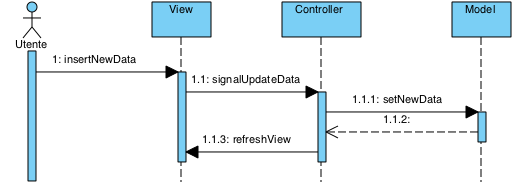
\includegraphics[width=0.8\linewidth]{./Content/Immagini/SimpleModelViewSequence.png}
		\caption{Diagramma di attività del pattern MVC}
		\label{img_MVCS}
	\end{figure}
	
	\begin{figure}[!h]
		\centering
		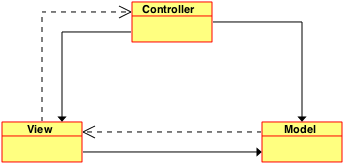
\includegraphics[width=0.8\linewidth]{./Content/Immagini/SimpleMVClassDiagram.png}
		\caption{Diagramma delle classi del pattern MVC}
		\label{img_MVCC}
	\end{figure}
	
\paragraph{Scopo dell'utilizzo:} viene utilizzato il design pattern\glossario{} MVC per mantenere separati i compiti dei diversi componenti software che interpretano i tre ruoli principali: Model View e Controller.
\paragraph{Contesto:} il pattern MVC viene utilizzato per l'architettura generale dell'applicazione. Viene utilizzato il sistema Signal e Slot di Qt\g{} descritto nella sezione \ref{signalslot} per far comunicare i componenti tra loro.
Ogni modifica fatta sulla View da parte dell'utente, viene inviata al Controller che da un comando al Model. Il Model notifica alla View ogni cambiamento e la View recupera i dati aggiornati del Model.

\pagebreak

\subsection{Design pattern creazionali}
\label{patt_creazionali}
%FACTORY
\subsubsection{Factory}
\label{creaz_factory}
\begin{figure}[!h]
	\centering
		\begin{subfigure}[b]{0.5\textwidth}
			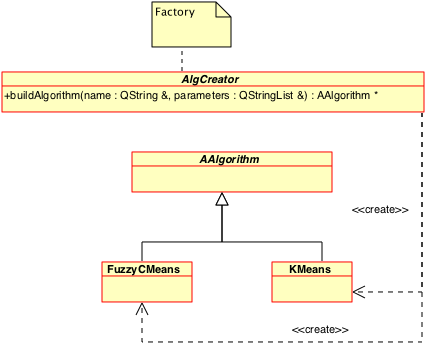
\includegraphics[width=\textwidth]{./Content/Immagini/FactoryAlg.png}
			\label{factoryalg}
			\caption{AlgCreator}
		\end{subfigure}
		
		\begin{subfigure}[b]{0.5\textwidth}
			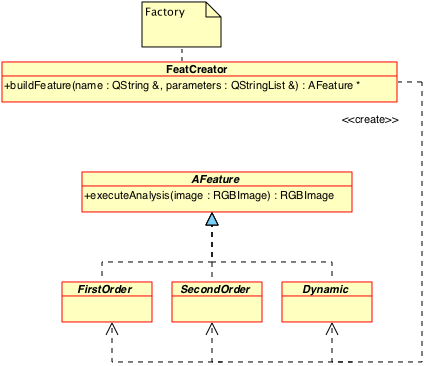
\includegraphics[width=\textwidth]{./Content/Immagini/FactoryFeatures.png}
			\label{factoryfeat}
			\caption{FeatCreator}
		\end{subfigure}
	\caption{Utilizzo di Factory in \project{}}
	\label{romeo_factory}
\end{figure}
\paragraph{Scopo dell'utilizzo:} viene utilizzato il design pattern\glossario{} Factory quando una classe non è a conoscenza di che tipo di oggetto sia necessario istanziare.
Le classi Factory hanno il compito di provvedere alla creazione di oggetti.
\\La scelta delle Concrete Product da creare verrà fatta in base ai parametri passati al metodo di creazione della classi Factory.
\paragraph{Contesto:} le classi che utilizzano tale pattern sono:
\begin{itemize}
	\item \verb!Romeo::Model::Core::FeatCreator! è Factory per tutte le classi (Concrete Product) che ereditano da \verb!Romeo::Model::Core::Features::AFeatures! (Product);
	\item \verb!Romeo::Model::Core::AlgCreator! è Factory per tutte le classi (Concrete Product) che ereditano da \verb!Romeo::Model::Core::Algorithms::AAlgorithm! (Product).
\end{itemize}
\pagebreak
%SINGLETON
\subsubsection{Singleton}
\label{creaz_singleton}
\begin{figure}[!h]
	\centering
	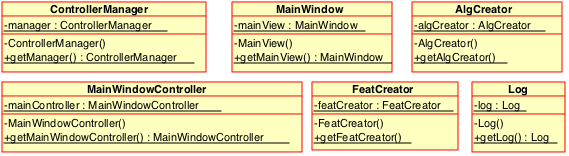
\includegraphics[width=1.1\linewidth]{./Content/Immagini/Singleton_dp.png}
	\caption{Utilizzo di Singleton in \project{}}
	\label{romeo_singleton}
\end{figure}
\paragraph{Scopo dell'utilizzo:} viene utilizzato il design pattern\glossario{} Singleton per garantire che durante l'esecuzione dell'applicazione esista una sola istanza della classe in questione.
\paragraph{Contesto:} le classi che necessitano di un'unica istanza sono:
\begin{itemize}
	\item \verb!Romeo::Controller::ControllerManager!;
	\item \verb!Romeo::View::Window::MainWindow!;
	\item \verb!Romeo::Controller::MainWindowController!;
	\item \verb!Romeo::Model::FacadeModel!;
	\item \verb!Romeo::Model::Core::AlgCreator!;
	\item \verb!Romeo::Model::Core::FeatCreator!;
\end{itemize}
\pagebreak
\subsection{Design pattern strutturali}
\label{patt_strutt}
%ADAPTER
\subsubsection{Adapter}
\label{strutt_ada}
\begin{figure}[!h]
		\centering
		\begin{subfigure}[b]{0.5\textwidth}
				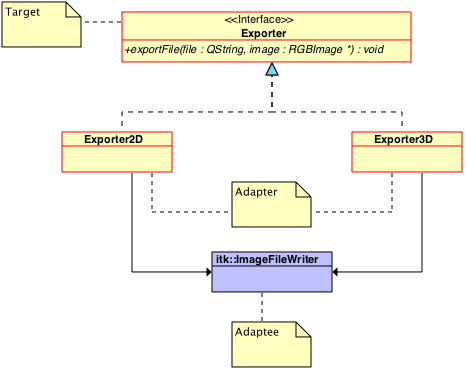
\includegraphics[width=1.2\textwidth]{./Content/Immagini/ExporterAdapter.png}
				\label{adapter}
				\caption{ExporterAdapter}
		\end{subfigure}
		\begin{subfigure}[b]{0.5\textwidth}
				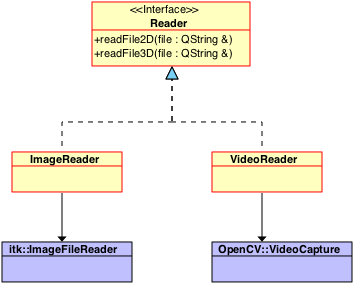
\includegraphics[width=1.2\textwidth]{./Content/Immagini/ReaderAdapter.png}
				\label{adapter}
				\caption{ReaderAdapter}
		\end{subfigure}
		\caption{Utilizzo Adapter in \project}
\end{figure}
\paragraph{Scopo dell'utilizzo:} il design pattern\g{} Adapter (Object Adapter ) viene utilizzato per convertire l'interfaccia di una classe in un'altra interfaccia richiesta dal client. In questo modo viene utilizzata un interfaccia stabile all'interno dell'applicativo.
 Nel nostro caso vengono adattate delle classi fornite dalla libreria esterna ITK\g{}. 
\paragraph{Contesto:} le classi che utilizzano tale pattern sono:
\begin{itemize}
	\item \verb!Romeo::Model::Util::ExporterModel::Exporter2D! adatta la classe \verb!itk::ImageFileWriter!;
	\item \verb!Romeo::Model::Util::ExporterModel::Exporter3D! adatta la classe \verb!itk::ImageFileWriter!;
	\item \verb!Romeo::Model::Util::ReaderModel::ImageReader! adatta la classe \verb!itk::VideoFileReader!;
	\item \verb!Romeo::Model::Util::ReaderModel::VideoReader! adatta la classe \verb!OpenCV::VideoCapture!;
	\item \verb!Romeo::Model::Core::InternalData2D! adatta la classe \verb!itk::Image!;
	\item \verb!Romeo::Model::Core::InternalData2D! adatta la classe \verb!itk::image!.
\end{itemize}


%DAO
\subsubsection{DAO (Data Access Object)}
\label{strutt_DAO}
\begin{figure}[!h]
		\centering
		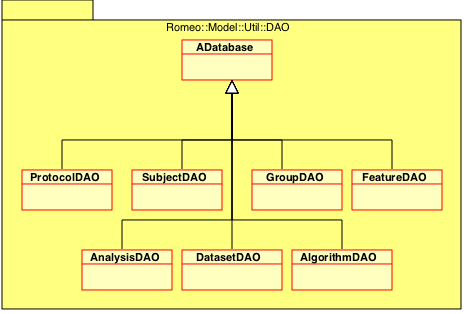
\includegraphics[width=0.7\linewidth]{./Content/Immagini/DAO_dp.png}
		\caption{Utilizzo di DAO in \project{}}
		\label{romeo_DAO}
\end{figure}
\paragraph{Scopo dell'utilizzo:} viene utilizzato il design pattern\glossario{} DAO per permettere l'interfacciamento al database.
\paragraph{Contesto:} le classi che utilizzano tale pattern sono:
\begin{itemize}
	\item \verb!Romeo::Model::Util::DAO::SubjectDAO!;
	\item \verb!Romeo::Model::Util::DAO::GroupDAO!;
	\item \verb!Romeo::Model::Util::DAO::DatasetDAO!;
	\item \verb!Romeo::Model::Util::DAO::ProtocolDAO!;
	\item \verb!Romeo::Model::Util::DAO::AlgorithmDAO!;
	\item \verb!Romeo::Model::Util::DAO::AnalysisDAO!;
	\item \verb!Romeo::Model::Util::DAO::FeatureDAO!.
\end{itemize}
\pagebreak
\subsubsection{Proxy}
\label{dp_proxy}
	\begin{figure}[!h]
		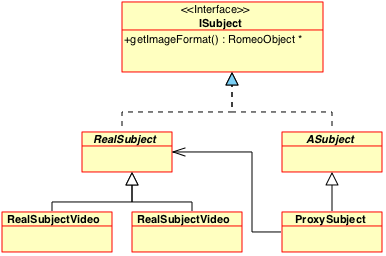
\includegraphics[width=0.7\linewidth]{./Content/Immagini/Proxy.png}
		\caption{Utilizzo di Proxy in \project{}}
		\label{proxy_romeo}
	\end{figure}
	\paragraph{Scopo dell'utilizzo:} viene utilizzato il design pattern\g{} per fornire un surrogato di un altro oggetto e per controllare l'accesso a tale oggetto.
	Tramite l'utilizzo di tale design pattern\g{} è possibile rimandare la creazione di oggetti costosi solo quando essi sono necessari. In \project{} non viene creato un oggetto RealSubject fino a chè non è necessario.
	\paragraph{Contesto:} le classi che utilizzano tale pattern sono:
		\begin{itemize}
			\item \verb!Romeo::Model::Core::ProxySubject!;
		\end{itemize}
\pagebreak

\subsection{Design pattern comportamentali}
\label{patt_comp}
%STRATEGY
\subsubsection{Strategy}
\label{comp_strat}
\begin{figure}[!h]
			\centering
			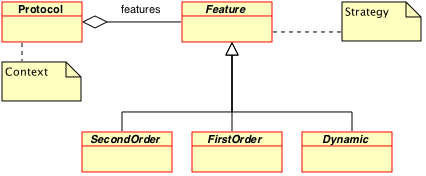
\includegraphics[width=0.6\linewidth]{./Content/Immagini/StrategyFeatures.png}
			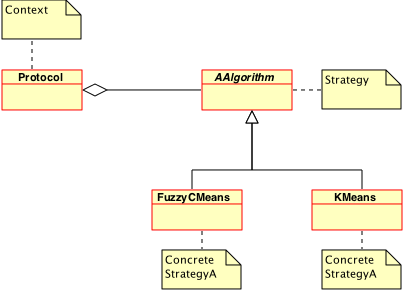
\includegraphics[width=0.6\linewidth]{./Content/Immagini/StrategyAlgorithms.png}
			\caption{Utilizzo di Strategy in \project{}}
		\label{romeo_strategy}
\end{figure}
\paragraph{Scopo dell'utilizzo:} viene utilizzato il design pattern\glossario{} Strategy per isolare algoritmi e renderli intercambiabili tra di loro. Tale pattern viene utilizzato per incapsulare gli algoritmi di clustering\g{} e le feature\g{} previste dai requisiti.
\\Si noti che per non appesantire troppo il diagramma non sono state riportare le Strategy concrete riguardanti le Feature\g{}.

\paragraph{Contesto:} le classi che utilizzano tale pattern sono:
\begin{itemize}
	\item \verb!Romeo::Model::Core::Algorithms::FuzzyCMeans!;
	\item \verb!Romeo::Model::Core::Algorithms::KMeans!;
	\item \verb!Romeo::Model::Core::Features::StdDeviationFeature!;
	\item \verb!Romeo::Model::Core::Features::SkewnessFeature!;
	\item \verb!Romeo::Model::Core::Features::KurtosisFeature!;
	\item \verb!Romeo::Model::Core::Features::MeanFeature!;
	\item \verb!Romeo::Model::Core::Features::CorrelationFeature!;
	\item \verb!Romeo::Model::Core::Features::EnergyFeature!;
	\item \verb!Romeo::Model::Core::Features::HomogeneityFeature!;
	\item \verb!Romeo::Model::Core::Features::EntropyFeature!;
	\item \verb!Romeo::Model::Core::Features::MeanDFeature!;
	\item \verb!Romeo::Model::Core::Features::MaximumFeature!;
	\item \verb!Romeo::Model::Core::Features::MinimumFeature!.
\end{itemize}